\chapter{Implementering}
I dette afsnit vil programmet blive beskrevet, i form af en overordnet programbeskrivelse og en dybdegående forklaring af programmets funktioner. Derudover vil der blive beskrevet hvordan brugeren interagere med programmet. 

\begin{wrapfigure}{r}{0.5\textwidth}
	\vspace{-40pt}
	\begin{center}
		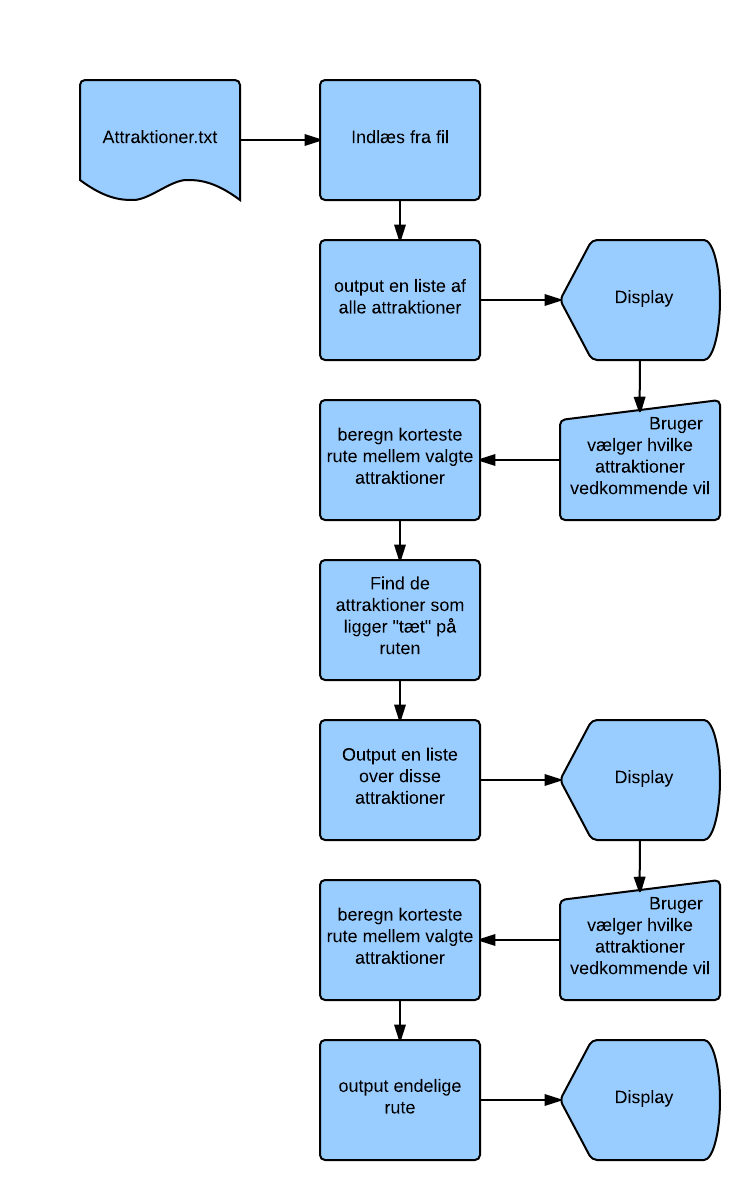
\includegraphics[scale=0.75]{program}\newline
		\textit{Figur 6.1: Flowchart over programmet}
	\end{center}
	\vspace{0pt}
	\vspace{0pt}
\end{wrapfigure}

\section{Programbeskrivelse}
Programmet begynder med at indlæse alle de forudbestemte tilgængelige attraktioner fra en tekstfil. Alle disse attraktioner bliver vist på en liste for brugeren i kommandoprompten med numre ud for hver attraktion. Brugeren vælger, hvilke attraktioner vedkommende har lyst til at besøge, ved at indtaste attraktionens nummer, hvor attraktionen så vil blive tilføjet til en liste. Denne liste kører gennem programmet, og den korteste rute bestemmes. Programmet tjekker derefter, for nærliggende attraktioner der kan tilføjes til ruten, på samme måde som i begyndelsen da de valgte attraktioner til deres rute. Hvis brugeren vælger ekstra attraktioner til deres rute, kører programmet igen, og den nye rute beregnes.  Når ruten er beregnet, vil ruten blive vist på skærmen, i den beregnede rækkefølge. Den samlede længde af ruten vil også blive vist.

\section{Beskrivelse af structs}
Til programmet bruges fire forskellige structs. Den første struct er "attraktion", som indeholder to strings, "navn" og "adresse", to doubles, "kmFraGreenwich" og "kmFraAekvator", og en int, "besoegt", der beskriver om attraktionen er besøgt eller ej. Denne struct bruges til at opdele og gemme de enkelte attraktioners data i programmet.\newline

\begin{lstlisting}
typedef struct {
char navn[MAX_STRING];
char adresse[MAX_STRING]; 
double kmFraGreenwich, kmFraAekvator;
int besoegt;
} attraktion;
\end{lstlisting} 

Næste struct er "naboRute", som indeholder en double, "ruteLaengde", og et array af attraktioner, "rute". Denne struct bruges til at lave ruter, hvor "rutelaengde" er længden af ruten og arrayet indeholder rækkefølgen af attraktioner på ruten. \newline

\begin{lstlisting}
typedef struct {
double ruteLaengde;
attraktion rute[ANTAL_ATTRAKTIONER];
} naboRute;
\end{lstlisting}

Næste struct er "kant", som indeholder to attraktioner, "startAttraktion" og "slutAttraktion", og en double, "laengde". Denne struct bliver brugt til at gemme data omkring afstanden mellem to punkter.\newline

\begin{lstlisting}
typedef struct {
attraktion start;
attraktion slut;
double laengde;
} kant;
\end{lstlisting}

Sidste struct er "vektor", som indeholder to doubles, "x" og "y". Denne struct bruges til at gemme x og y koordinater for vektorer og i nogle tilfælde punkter. \newline

\begin{lstlisting}
typedef struct {
double x, y;
} vektor;
\end{lstlisting}

\section{Beskrivelse af funktioner}
Attraktionerne til programmet bliver indlæst fra en .txt fil når programmet køres. I programmet bliver filen indlæst i en funktion som hedder initialiserAttraktioner. Hvis filen ikke er tom vil elementerne, vha. funktionen fscanf, blive indlæst i grupper af 4, hvor de bliver indlæst som ”attraktion” hvilket er defineret som et struct. Hvis filen er tom, vil en advarsel blive vist i prompten og lukke programmet ned. Når alt information er indlæst fra filen, og den ikke længere er nødvendig, lukkes filen.\newline

\begin{lstlisting}
void initialiserAttraktioner(attraktion *attraktioner){
FILE *input_file_pointer;
int i = 0;
double lndgrad;
double brdgrad;

input_file_pointer = fopen("attraktioner.txt", "r");

if(input_file_pointer != NULL){
while(fscanf(input_file_pointer, " %s %s %lf %lf", attraktioner[i].navn, attraktioner[i].adresse, &brdgrad, &lndgrad) == 4){
attraktioner[i].kmFraGreenwich = lndgrad * KM_PR_LNDGRAD;
attraktioner[i].kmFraAekvator = brdgrad * KM_PR_BRDGRAD;
attraktioner[i].besoegt = 0;
i++;
}
}else{
printf("kunne ikke aabne fil\n"); exit(1);
}
fclose(input_file_pointer);
} 
\end{lstlisting}

Funktionen ”udregn\_kanter” bruges til at udregne distancen mellem punkterne. Beregningen af distancerne sker vha. ”beregn\_dist”, ved at sende en start og slut attraktion. Derefter bliver start- og slut attraktionen plus længden imellem dem lagt ind som en kant i kanter arrayet. Dette gøres i en for-løkke i en anden for-løkke, hvor der for hvert punkt bliver der udregnet distancen til de punkter der ikke allerede er blevet oprettet en kant for, i en tidligere iteration af løkkerne. For hver kant der bliver oprettet, oprettes en ekstra kant som har samme længde, men har modsat start og slut attraktion. Så hvis der oprettes en kant fra x til y, vil der også blive oprettet en kant fra y til x, med samme længde. Kanterne bliver tilføjet til kantarrayet, gennem den pointer der er inputparameter til funktionen, så kanterne kan blive tilgået fra resten af programmet. \newline

\begin{lstlisting}
void udregn_kanter(attraktion *attraktioner, kant *kanter)
{
int i;
int y;
int indexTilKanter = 0;
for (i = 0; i < ANTAL_ATTRAKTIONER; i++)
{
for (y = i; y < ANTAL_ATTRAKTIONER; y++)
{
if (strcmp(attraktioner[i].navn, attraktioner[y].navn) != 0)
{
kant k, j;
k.start = attraktioner[i];
j.slut = k.start;
k.slut = attraktioner[y];
j.start = k.slut;
k.laengde = beregn_dist(k.start, k.slut);
j.laengde = k.laengde;
kanter[indexTilKanter] = k;
kanter[indexTilKanter+1] = j;
indexTilKanter += 2;
}
}
}
}
\end{lstlisting}

Funktionen ”beregn\_dist” er en implementering af pythagoras sætning til at finde længden mellem 2 punkter. Funktionen returnere den beregnede distance mellem de to attraktioner. \newline

\begin{lstlisting}
double beregn_dist(attraktion startAttraktion, attraktion slutAttraktion)
{
return sqrt(pow(startAttraktion.kmFraGreenwich - slutAttraktion.kmFraGreenwich, 2) + 
pow(startAttraktion.kmFraAekvator - slutAttraktion.kmFraAekvator, 2));
}
\end{lstlisting}

\begin{wrapfigure}{r}{0.5\textwidth}
	\vspace{0pt}
	\begin{center}
		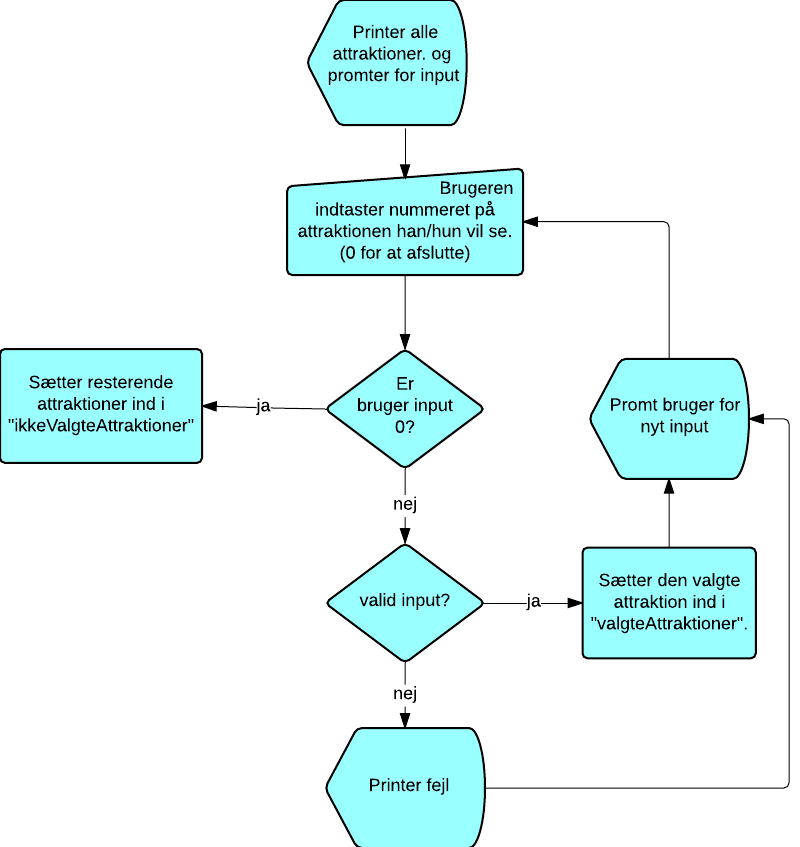
\includegraphics[scale=0.7]{valgAfAttraktioner}\newline
		\textit{Figur 6.2: Flowchart over “valgafAttraktioner” funktionen}
	\end{center}
	\vspace{0pt}
	\vspace{0pt}
\end{wrapfigure}

Brugeren bliver præsenteret for en liste over alle tilgængelige attraktioner fra inputparameteren, og attraktionernes tilhørende nummer i funktionen "valgafAttraktioner. Brugeren bliver bedt om at indtaste attraktionernes matchende numre, hvilket vil blive tilføjet til en list. Taster brugeren 0, bliver brugeren præsentere for sine valg, og beregninger af den korteste rute igangsættes. Programmet returnere listen af valgte attraktioner. \newline

\begin{lstlisting}
void valgafAttraktioner(attraktion *attraktioner, 
attraktion *valgteAttraktioner, 
int *antalValgteAttraktioner, 
attraktion *ikkeValgteAttraktioner){
int i = 0, j = 0, k = 0, l = 0, 
m = 0, n = 0, o = 0, valgt = 0;

for(i = 0; i < ANTAL_ATTRAKTIONER; i++){
printf("%d: %s\n", i+1, attraktioner[i].navn);
}

printf("vaelg de attraktioner du oensker 
		at se ved at skrive det tilhoerende tal.\n");
printf("vaelg et tal (svarende til en attraktion) 
		af gangen og tryk enter efter 
		hver indtastet tal\n");
printf("indtast ikke samme tal 2 gange\n");
do{
if(scanf("%d", &k) != 1){
printf("Fejl i indlaesning. Farvel.\n"); exit(0);
}
if(k != 0){
valgteAttraktioner[j] = attraktioner[k-1];
j++;
}
} while(j < ANTAL_ATTRAKTIONER && k != 0);

for (l = 0; l < ANTAL_ATTRAKTIONER; ++l)
{
valgt = 0;
for (m = 0; m < j; ++m)
{
if(strcmp(attraktioner[l].navn, 
   valgteAttraktioner[m].navn) == 0){
m = j;
valgt = 1;
}	
}
if(valgt != 1){
ikkeValgteAttraktioner[n] = attraktioner[l];
n++;
}
}
*antalValgteAttraktioner = j;
}
\end{lstlisting}


Funktionen ”findNaboRute” benytter NNA (Nearest Neighbour Algorithm, eller Nærmeste Nabo Algoritme), til at finde den korteste rute mellem en række attraktioner for et bestemt startsted, der er angivet i inputparametrene. Efter at have fundet den korteste rute ud fra NNA som beskrevet i teoriafsnittet 5.1.1 om grafteori, returnere den et array med ruten og distancen for denne rute. \newline
\begin{flushleft}
	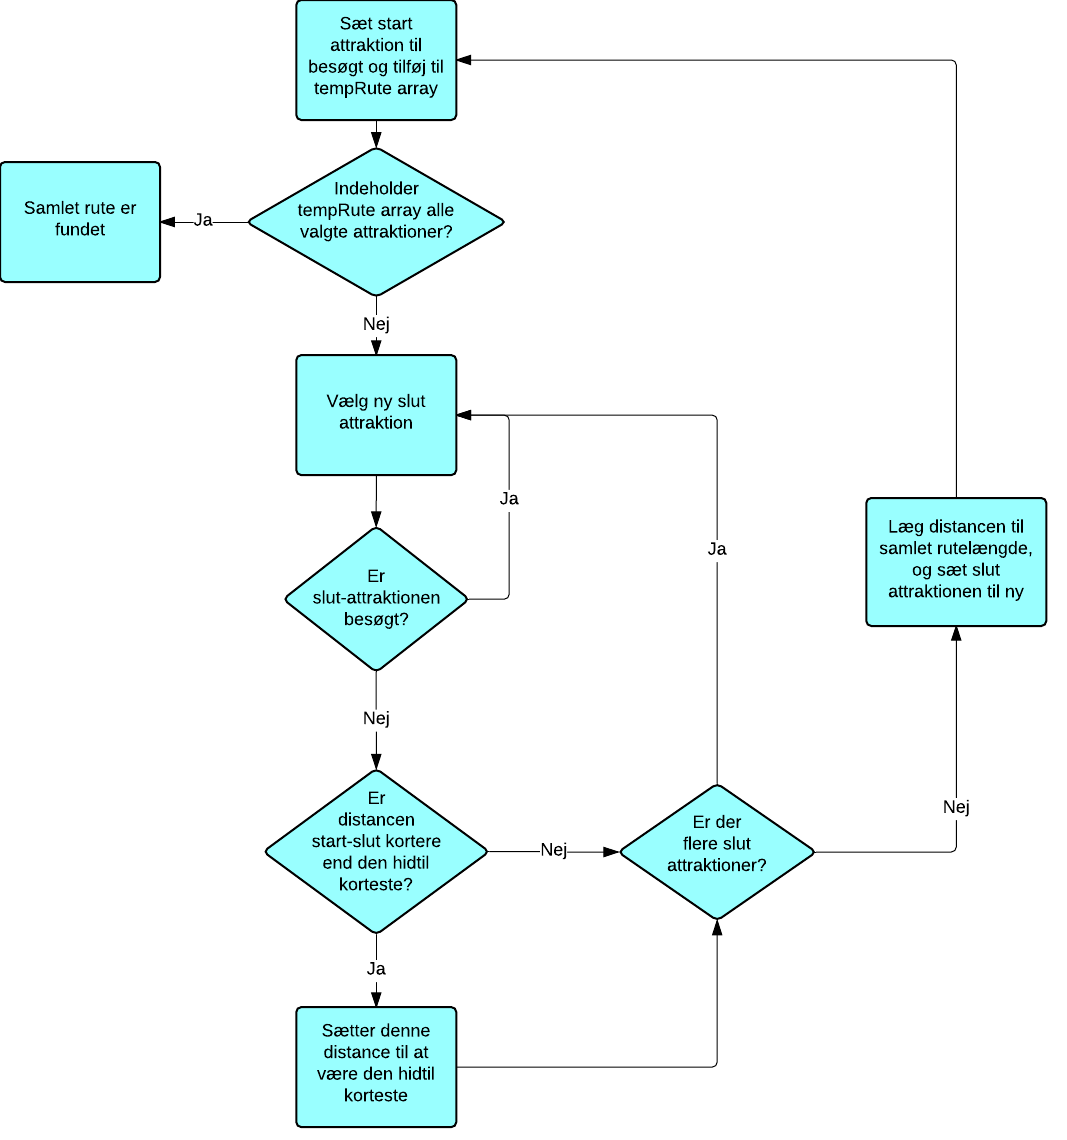
\includegraphics[scale=0.6]{findnaborute}\newline
	\textit{Figur 6.3: Flowchart over “findNaboRute” funktionen”}
\end{flushleft}
\begin{lstlisting}
void findNaboRute(attraktion *valgteAttraktioner, 
int antalValgteAttraktioner, attraktion *startAttraktion, kant *kanter, attraktion **tempRute, double *ruteLaengde){
int i = 0;
double lavesteLaengde = 10000;
*ruteLaengde = 0;

tempRute[i] = startAttraktion;

for(i = 0; i < antalValgteAttraktioner-1; ++i){ /*da der f.eks. kun er 4 kanter imellem 5 punkter*/
tempRute[i]->besoegt = 1;
int j = 0;
for (j = 0; j < antalValgteAttraktioner; ++j){
if(valgteAttraktioner[j].besoegt != 1 && findDist(*tempRute[i], valgteAttraktioner[j], kanter) < lavesteLaengde){
lavesteLaengde = findDist(*tempRute[i],valgteAttraktioner[j], kanter);
tempRute[i+1] = &valgteAttraktioner[j];
}
}
*ruteLaengde += lavesteLaengde;
lavesteLaengde = 10000;
}
tempRute[antalValgteAttraktioner] 
= startAttraktion;
*ruteLaengde += findDist(*tempRute[antalValgteAttraktioner-1], *tempRute[antalValgteAttraktioner], kanter);
}
\end{lstlisting}

”findKortesteNaboRute” benytter funktionen ”findNaboRute”, til at finde ud af hvilket startsted der giver den korteste rute. Dette gøres ved at sætte en variable til en stor værdi, som rutedistancen ikke vil gå over, og opdatere den hvis ”findNaboRute” returnere en distance for ruten gennem de givne attraktioner med en given start attraktion, der er lavere end de foregående ruter. ”findKortesteNaboRute” returnere et array med den korteste rute, og den samlede længde af denne rute.  \newline
\begin{flushleft}
	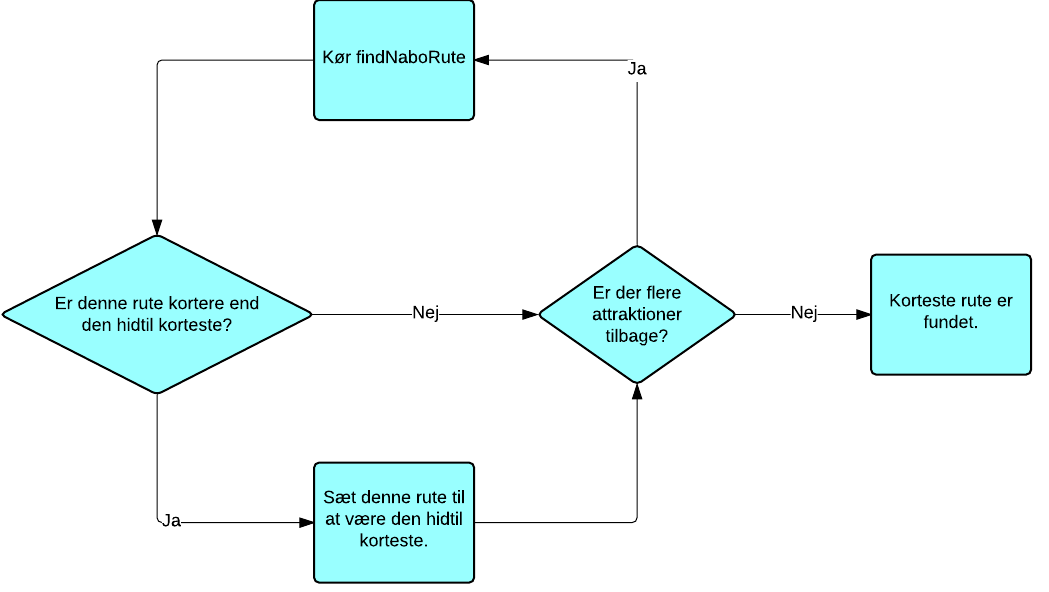
\includegraphics[scale=0.6]{findKortesteNaboRute}\newline
	\textit{Figur 6.3: Flowchart over “findKortesteNaboRute” funktionen”}
\end{flushleft}
\begin{lstlisting}
void findKortesteNaboRute(attraktion
*valgteAttraktioner, 
int antalValgteAttraktioner, 
attraktion *ruteAttraktioner, kant *kanter, 
double *samletLaengde){
/* indput er valgteAttraktioner arrayet, 
og kanter arrayet*/
/*output er ruteAttraktioner og samletLaengde*/
double ruteLaengde;
attraktion *tempRute[antalValgteAttraktioner+1];
*samletLaengde = 100000;

int i;
int h;
int j;
for (i = 0; i < antalValgteAttraktioner; ++i){
for (h = 0; h < antalValgteAttraktioner; ++h){
valgteAttraktioner[h].besoegt = 0;
}
findNaboRute(valgteAttraktioner,
antalValgteAttraktioner, 
&valgteAttraktioner[i], kanter, tempRute,
&ruteLaengde);
if(ruteLaengde < *samletLaengde){
*samletLaengde = ruteLaengde;
for (j = 0; j < antalValgteAttraktioner+1; ++j)
{
ruteAttraktioner[j] = *tempRute[j];
}
}
}
}
\end{lstlisting}

Funktionen "findDist" gennemgår alle kanter der allerede er oprettet, og returnere distancen mellem to attraktioner, som er sendt med kaldet af funktionen, uden at skulle beregne den igen. \newline

\begin{lstlisting}
double findDist(attraktion start, attraktion slut, kant *kanter){
int i;
for (i = 0; i < ANTAL_KANTER; ++i)
{
if(strcmp(kanter[i].start.navn, start.navn) == 0 && strcmp(kanter[i].slut.navn, slut.navn) == 0){
return kanter[i].laengde;
}
}
printf("Kunne ikke finde passende kant\n"); exit(0);
}
\end{lstlisting}

Funktionen ”attraktionErTilfoejet” bruges til at finde ud af, om en attraktioner allerede er tilføjet til ens liste over ekstra attraktioner, og returnere enten true eller false. \newline

\begin{lstlisting}
int attraktionErTilfoejet(attraktion *ekstraAttraktioner, int antalEsktraAttraktioner, attraktion attraktionAtTilfoeje){
int i;
for (i = 0; i < antalEsktraAttraktioner; ++i)
{
if(strcmp(ekstraAttraktioner[i].navn, attraktionAtTilfoeje.navn) == 0){
return 1;
}
}
return 0;
}
\end{lstlisting}

Funktionen ”prikProdukt” bruges til at finde prikproduktet mellem to vektorer, hvilket også er det funktionen returnere. \newline

\begin{lstlisting}
double prikProdukt(vektor vektor1, vektor vektor2){
return (vektor1.x * vektor2.x) + (vektor1.y * vektor2.y);
}
\end{lstlisting}

Funktionen ”findEkstraAttraktionerFirkant” benytter beregningerne fra teoriafsnittet "Vektorteori", til at finde ud af om der findes en evt. interessant attraktion på brugerens rute. Der tjekkes om attraktionAtTilfoeje ligger inden for en bestemt distance til linjen mellem start og slut punkter. Hvis attraktionAtTilfoeje ligger indenfor, bliver den lagt i ekstraAttraktioner arrayet. \newline

\begin{lstlisting}
void findEkstraAttraktionerFirkant(attraktion startAttraktion, attraktion slutAttraktion, attraktion *valgteAttraktioner, 
int *antalValgteAttraktioner, kant *kanter, attraktion attraktionAtTilfoeje, double maxDist, 
attraktion *ekstraAttraktioner, int *antalEsktraAttraktioner){
int i, j;
double vektorLaengde;
vektor ruteVektor, ruteVinkelretVektor, ruteEnhedsVinkelretVektor, mainHjoerne, side1Vektor, side2Vektor, punktVektor;

vektorLaengde = findDist(startAttraktion, slutAttraktion, kanter);
ruteVektor.x = slutAttraktion.kmFraGreenwich - startAttraktion.kmFraGreenwich;
ruteVektor.y = slutAttraktion.kmFraAekvator - startAttraktion.kmFraAekvator;
ruteVinkelretVektor.x = -ruteVektor.y;
ruteVinkelretVektor.y = ruteVektor.x;
ruteEnhedsVinkelretVektor.x = ruteVinkelretVektor.x / vektorLaengde;
ruteEnhedsVinkelretVektor.y = ruteVinkelretVektor.y / vektorLaengde;
mainHjoerne.x = startAttraktion.kmFraGreenwich + ruteEnhedsVinkelretVektor.x * maxDist;
mainHjoerne.y = startAttraktion.kmFraAekvator + ruteEnhedsVinkelretVektor.y * maxDist;
side1Vektor.x = ruteVektor.x;
side1Vektor.y = ruteVektor.y;
side2Vektor.x = -2 * ruteEnhedsVinkelretVektor.x * maxDist;
side2Vektor.y = -2 * ruteEnhedsVinkelretVektor.y * maxDist;

punktVektor.x = attraktionAtTilfoeje.kmFraGreenwich - mainHjoerne.x;
punktVektor.y = attraktionAtTilfoeje.kmFraAekvator - mainHjoerne.y;
if(0 < prikProdukt(punktVektor, side1Vektor) && prikProdukt(punktVektor, side1Vektor) < prikProdukt(side1Vektor, side1Vektor) &&
0 < prikProdukt(punktVektor, side2Vektor) && prikProdukt(punktVektor, side2Vektor) < prikProdukt(side2Vektor, side2Vektor)){
ekstraAttraktioner[*antalEsktraAttraktioner] = attraktionAtTilfoeje;
*antalEsktraAttraktioner += 1;
}
}
\end{lstlisting}

For at foreslå ekstra attraktioner til den valgte rute, bruges funktionen ”findEkstraAttraktioner”, hvor dette vil udgøre den interessante rute. Dette gøres den ved først at bruge funktionen ”findDist”, til at finde ikke valgte attraktioner inden for en bestemt distance af de valgte attraktioner. Er en attraktion ikke inden for denne radius, bruges funktionen ”findEkstraAttraktionerFirkant” for at finde ud af, om attraktionen ligger tæt på ruten mellem to attraktioner. De attraktioner der enten er inden for den bestemte distance af enten attraktionerne eller ruterne derimellem, tilføjes til et array der returneres fra funktionen. \newline

\begin{lstlisting}
void findEkstraAttraktioner(attraktion *ruteAttraktioner, attraktion *valgteAttraktioner, int *antalValgteAttraktioner, 
kant *kanter, attraktion *ikkeValgteAttraktioner, double maxDist, attraktion *ekstraAttraktioner, int *antalEsktraAttraktioner){

int i, j, antalIkkeValgteAttraktioner = ANTAL_ATTRAKTIONER - *antalValgteAttraktioner;

for (i = 0; i < *antalValgteAttraktioner; ++i)
{
for (j = 0; j < antalIkkeValgteAttraktioner; ++j)
{

if(attraktionErTilfoejet(ekstraAttraktioner, *antalEsktraAttraktioner, ikkeValgteAttraktioner[j])){
}else if(findDist(ruteAttraktioner[i], ikkeValgteAttraktioner[j], kanter) < maxDist || 
findDist(ruteAttraktioner[i+1], ikkeValgteAttraktioner[j], kanter) < maxDist){
ekstraAttraktioner[*antalEsktraAttraktioner] = ikkeValgteAttraktioner[j];
*antalEsktraAttraktioner += 1;
}else{
findEkstraAttraktionerFirkant(ruteAttraktioner[i], ruteAttraktioner[i+1], valgteAttraktioner, antalValgteAttraktioner,
kanter, ikkeValgteAttraktioner[j], maxDist, ekstraAttraktioner, antalEsktraAttraktioner);
}
}
}
}
\end{lstlisting}

Funktionen ”aendre\_startsted”, tager en rute som inputparameter, sammen med det startsted der ønskes. Funktionen laver derefter et nyt array, der har det nye startsted som første og sidste element, så ruten starter i startstedet, og vender tilbage dertil. Dette array er hvad funktionen returnere.  \newline

\begin{lstlisting}
void aendre_startsted(attraktion *ruten, attraktion nytStartSted, int antalAttraktioner, attraktion *outputRute)
{
int i = 0, startStedIndex = 0;

for (i = 0; i < antalAttraktioner; i++)
{
if (strcmp(ruten[i].navn, nytStartSted.navn) == 0)
startStedIndex = i;
}

for (i = 0; i < antalAttraktioner; i++)
{

if (startStedIndex == antalAttraktioner-1)
{
startStedIndex = 1;
outputRute[i] = ruten[0];
}
else
{
outputRute[i] = ruten[startStedIndex];
startStedIndex++;
}
}
}
\end{lstlisting}

